\documentclass{standalone}
\usepackage{tikz}
\usetikzlibrary{patterns, positioning}
\usepackage[sfdefault]{ClearSans} %% option 'sfdefault' activates Clear Sans as the default text font
\usepackage[T1]{fontenc}

\begin{document}
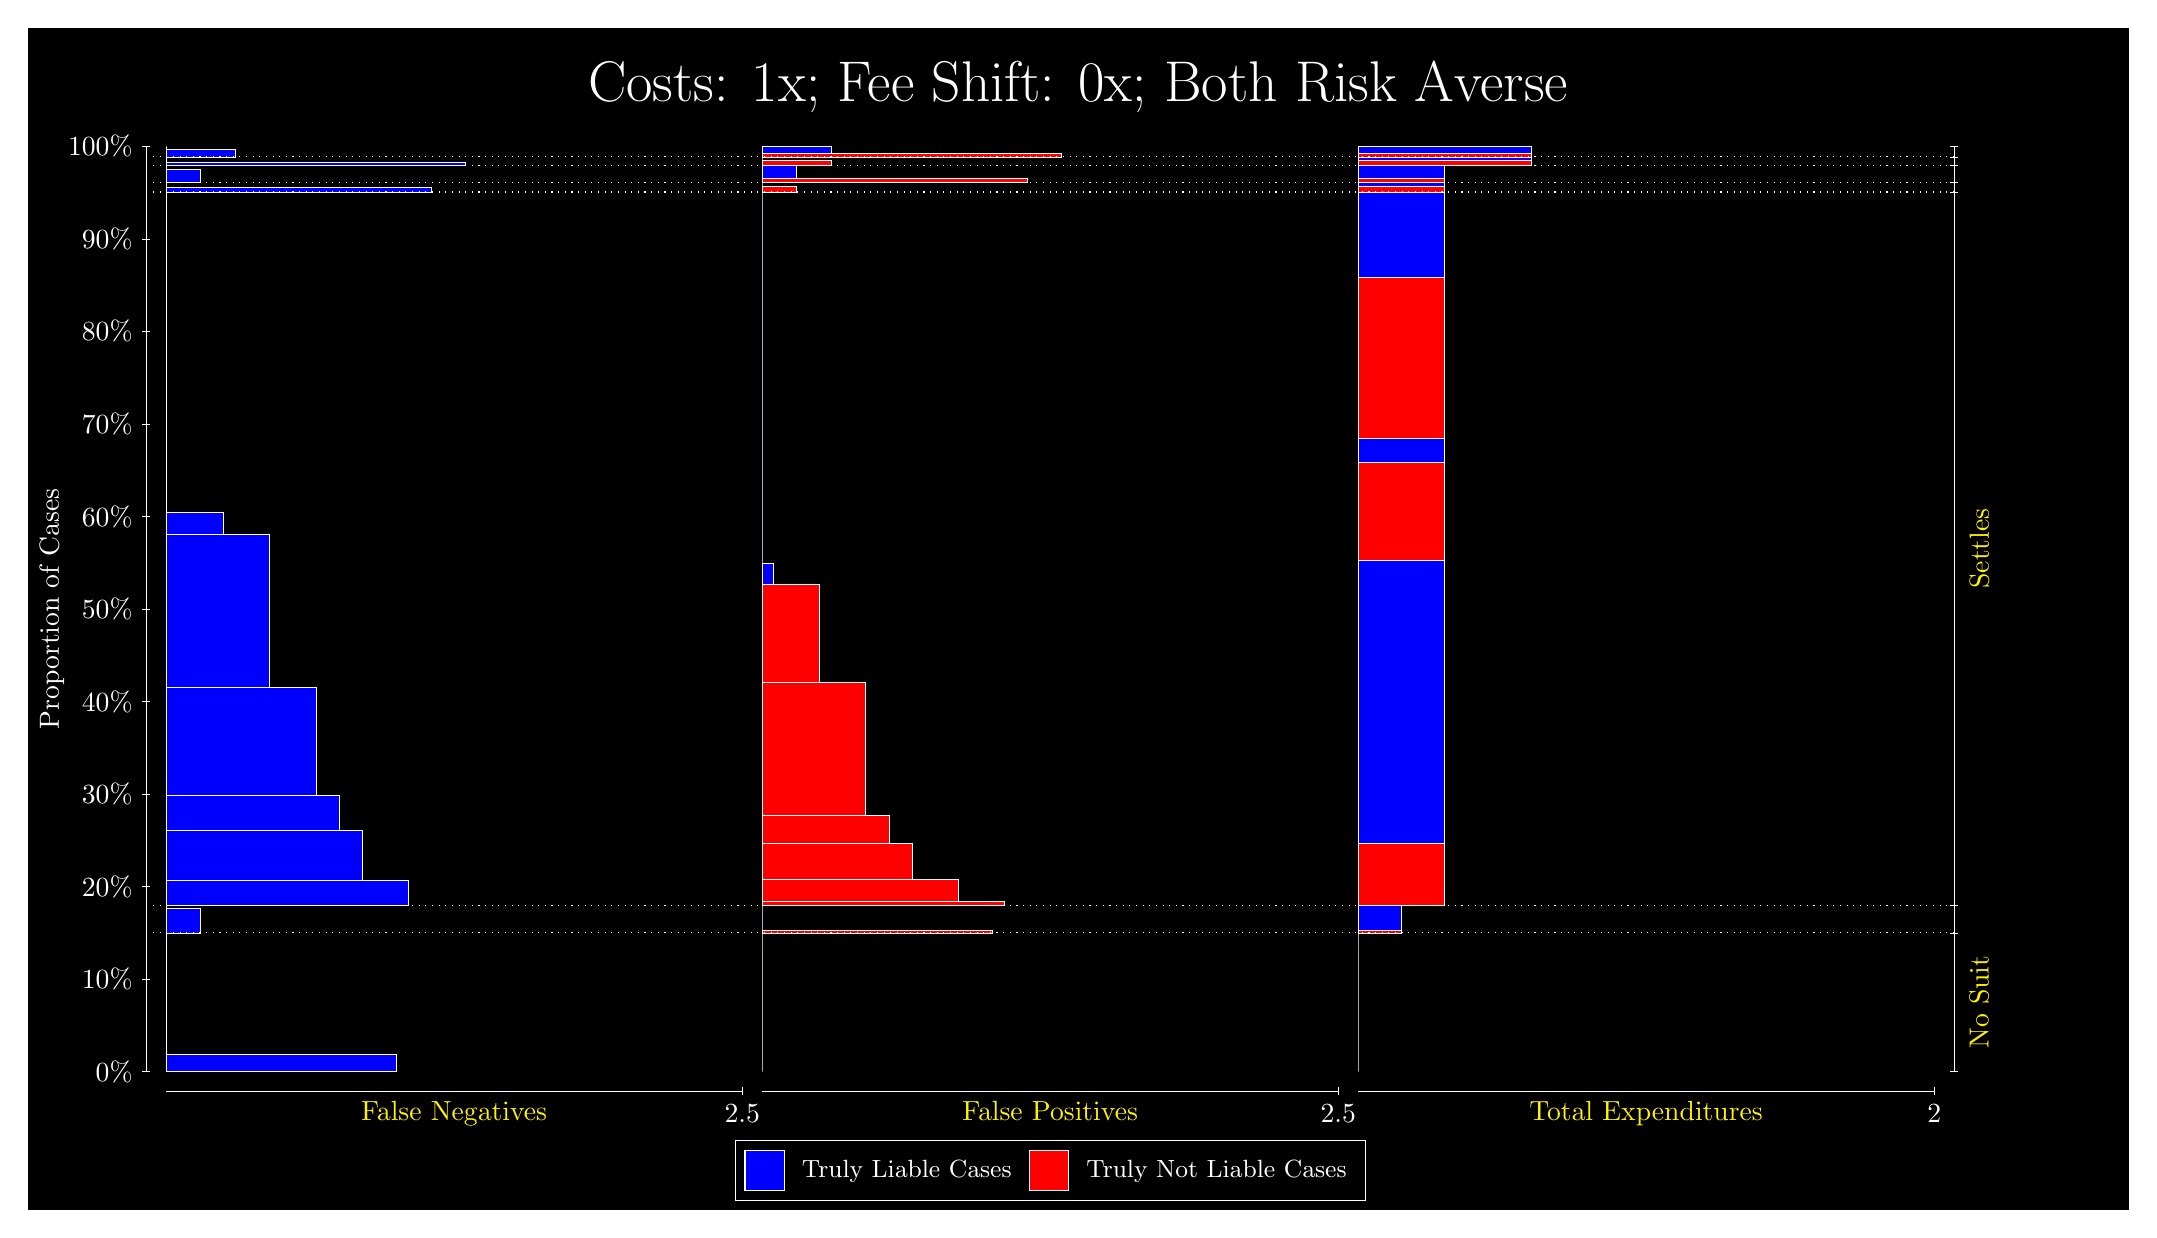
\begin{tikzpicture}
\draw[fill=black] (0,0) rectangle (26.667,15);
\draw[text=white] (0,13.5) rectangle (26.667,15) node[midway] {\huge Costs: 1x; Fee Shift: 0x; Both Risk Averse};
\draw[white, very thin] (1.5,1.75) -- (1.5,13.5);
\node[rotate=90, text=white, anchor=center] at (0.3, 7.625) {Proportion of Cases};
\draw[white, very thin] (1.45,1.75) -- (1.55,1.75);
\node[text=white, anchor=east] at (1.45, 1.75) {0\%};
\draw[white, very thin] (1.45,2.925) -- (1.55,2.925);
\node[text=white, anchor=east] at (1.45, 2.925) {10\%};
\draw[white, very thin] (1.45,4.1) -- (1.55,4.1);
\node[text=white, anchor=east] at (1.45, 4.1) {20\%};
\draw[white, very thin] (1.45,5.275) -- (1.55,5.275);
\node[text=white, anchor=east] at (1.45, 5.275) {30\%};
\draw[white, very thin] (1.45,6.45) -- (1.55,6.45);
\node[text=white, anchor=east] at (1.45, 6.45) {40\%};
\draw[white, very thin] (1.45,7.625) -- (1.55,7.625);
\node[text=white, anchor=east] at (1.45, 7.625) {50\%};
\draw[white, very thin] (1.45,8.8) -- (1.55,8.8);
\node[text=white, anchor=east] at (1.45, 8.8) {60\%};
\draw[white, very thin] (1.45,9.975) -- (1.55,9.975);
\node[text=white, anchor=east] at (1.45, 9.975) {70\%};
\draw[white, very thin] (1.45,11.15) -- (1.55,11.15);
\node[text=white, anchor=east] at (1.45, 11.15) {80\%};
\draw[white, very thin] (1.45,12.325) -- (1.55,12.325);
\node[text=white, anchor=east] at (1.45, 12.325) {90\%};
\draw[white, very thin] (1.45,13.5) -- (1.55,13.5);
\node[text=white, anchor=east] at (1.45, 13.5) {100\%};

\draw[white, very thin] (24.457,1.75) -- (24.457,13.5);
\draw[white, very thin] (24.407,1.75) -- (24.507,1.75);
\node[anchor=west] at (24.407, 1.75) {};
\draw[white, very thin] (24.407,3.5119) -- (24.507,3.5119);
\node[anchor=west] at (24.407, 3.5119) {};
\draw[white, very thin] (24.407,3.8631) -- (24.507,3.8631);
\node[anchor=west] at (24.407, 3.8631) {};
\draw[white, very thin] (24.407,12.92) -- (24.507,12.92);
\node[anchor=west] at (24.407, 12.92) {};
\draw[white, very thin] (24.407,13.046) -- (24.507,13.046);
\node[anchor=west] at (24.407, 13.046) {};
\draw[white, very thin] (24.407,13.256) -- (24.507,13.256);
\node[anchor=west] at (24.407, 13.256) {};
\draw[white, very thin] (24.407,13.367) -- (24.507,13.367);
\node[anchor=west] at (24.407, 13.367) {};
\draw[white, very thin] (24.407,13.5) -- (24.507,13.5);
\node[anchor=west] at (24.407, 13.5) {};

\draw[white, very thin, fill=blue] (1.75,1.75) rectangle (4.6775,1.9736);
\draw[white, very thin, fill=red] (1.75,1.9736) rectangle (1.75,3.5119);
\draw[white, very thin, fill=blue] (1.75,3.5119) rectangle (2.1891,3.8293);
\draw[white, very thin, fill=red] (1.75,3.8293) rectangle (1.75,3.8631);
\draw[white, very thin, fill=blue] (1.75,3.8631) rectangle (4.8239,4.1752);
\draw[white, very thin, fill=blue] (1.75,4.1752) rectangle (4.2384,4.8149);
\draw[white, very thin, fill=blue] (1.75,4.8149) rectangle (3.9457,5.2521);
\draw[white, very thin, fill=blue] (1.75,5.2521) rectangle (3.6529,6.6331);
\draw[white, very thin, fill=blue] (1.75,6.6331) rectangle (3.0674,8.5735);
\draw[white, very thin, fill=blue] (1.75,8.5735) rectangle (2.4819,8.8467);
\draw[white, very thin, fill=red] (1.75,8.8467) rectangle (1.75,12.92);
\draw[white, very thin, fill=blue] (1.75,12.92) rectangle (5.1167,12.977);
\draw[white, very thin, fill=red] (1.75,12.977) rectangle (1.75,13.046);
\draw[white, very thin, fill=blue] (1.75,13.046) rectangle (2.1891,13.206);
\draw[white, very thin, fill=red] (1.75,13.206) rectangle (1.75,13.256);
\draw[white, very thin, fill=blue] (1.75,13.256) rectangle (5.5558,13.298);
\draw[white, very thin, fill=red] (1.75,13.298) rectangle (1.75,13.367);
\draw[white, very thin, fill=blue] (1.75,13.367) rectangle (2.6283,13.458);
\draw[white, very thin, fill=red] (1.75,13.458) rectangle (1.75,13.5);
\draw[white, very thin, fill=red] (9.3189,1.75) rectangle (9.3189,3.2883);
\draw[white, very thin, fill=blue] (9.3189,3.2883) rectangle (9.3189,3.5119);
\draw[white, very thin, fill=red] (9.3189,3.5119) rectangle (12.246,3.5456);
\draw[white, very thin, fill=blue] (9.3189,3.5456) rectangle (9.3189,3.8631);
\draw[white, very thin, fill=red] (9.3189,3.8631) rectangle (12.393,3.9143);
\draw[white, very thin, fill=red] (9.3189,3.9143) rectangle (11.807,4.1884);
\draw[white, very thin, fill=red] (9.3189,4.1884) rectangle (11.222,4.6495);
\draw[white, very thin, fill=red] (9.3189,4.6495) rectangle (10.929,5.0027);
\draw[white, very thin, fill=red] (9.3189,5.0027) rectangle (10.636,6.6987);
\draw[white, very thin, fill=red] (9.3189,6.6987) rectangle (10.051,7.9361);
\draw[white, very thin, fill=blue] (9.3189,7.9361) rectangle (9.4652,8.2093);
\draw[white, very thin, fill=blue] (9.3189,8.2093) rectangle (9.3189,12.92);
\draw[white, very thin, fill=red] (9.3189,12.92) rectangle (9.758,12.988);
\draw[white, very thin, fill=blue] (9.3189,12.988) rectangle (9.3189,13.046);
\draw[white, very thin, fill=red] (9.3189,13.046) rectangle (12.686,13.096);
\draw[white, very thin, fill=blue] (9.3189,13.096) rectangle (9.758,13.256);
\draw[white, very thin, fill=red] (9.3189,13.256) rectangle (10.197,13.325);
\draw[white, very thin, fill=blue] (9.3189,13.325) rectangle (9.3189,13.367);
\draw[white, very thin, fill=red] (9.3189,13.367) rectangle (13.125,13.409);
\draw[white, very thin, fill=blue] (9.3189,13.409) rectangle (10.197,13.5);
\draw[white, very thin, fill=red] (16.888,1.75) rectangle (16.888,3.2883);
\draw[white, very thin, fill=blue] (16.888,3.2883) rectangle (16.888,3.5119);
\draw[white, very thin, fill=red] (16.888,3.5119) rectangle (17.437,3.5456);
\draw[white, very thin, fill=blue] (16.888,3.5456) rectangle (17.437,3.8631);
\draw[white, very thin, fill=red] (16.888,3.8631) rectangle (17.986,4.6495);
\draw[white, very thin, fill=blue] (16.888,4.6495) rectangle (17.986,8.2441);
\draw[white, very thin, fill=red] (16.888,8.2441) rectangle (17.986,9.4815);
\draw[white, very thin, fill=blue] (16.888,9.4815) rectangle (17.986,9.7936);
\draw[white, very thin, fill=red] (16.888,9.7936) rectangle (17.986,11.843);
\draw[white, very thin, fill=blue] (16.888,11.843) rectangle (17.986,12.92);
\draw[white, very thin, fill=red] (16.888,12.92) rectangle (17.986,12.988);
\draw[white, very thin, fill=blue] (16.888,12.988) rectangle (17.986,13.046);
\draw[white, very thin, fill=red] (16.888,13.046) rectangle (17.986,13.096);
\draw[white, very thin, fill=blue] (16.888,13.096) rectangle (17.986,13.256);
\draw[white, very thin, fill=red] (16.888,13.256) rectangle (19.083,13.325);
\draw[white, very thin, fill=blue] (16.888,13.325) rectangle (19.083,13.367);
\draw[white, very thin, fill=red] (16.888,13.367) rectangle (19.083,13.409);
\draw[white, very thin, fill=blue] (16.888,13.409) rectangle (19.083,13.5);
\draw[white, dotted] (1.5,3.5119) -- (24.457,3.5119);
\draw[white, dotted] (1.5,3.8631) -- (24.457,3.8631);
\draw[white, dotted] (1.5,12.92) -- (24.457,12.92);
\draw[white, dotted] (1.5,13.046) -- (24.457,13.046);
\draw[white, dotted] (1.5,13.256) -- (24.457,13.256);
\draw[white, dotted] (1.5,13.367) -- (24.457,13.367);
\draw[white, very thin] (1.75,1.5) -- (9.0689,1.5);
\node[text=yellow, anchor=north] at (5.4094, 1.5) {False Negatives};
\draw[white, very thin] (9.0689,1.45) -- (9.0689,1.55);
\node[text=white, anchor=north] at (9.0689, 1.45) {2.5};

\draw[white, very thin] (9.3189,1.5) -- (16.638,1.5);
\node[text=yellow, anchor=north] at (12.978, 1.5) {False Positives};
\draw[white, very thin] (16.638,1.45) -- (16.638,1.55);
\node[text=white, anchor=north] at (16.638, 1.45) {2.5};

\draw[white, very thin] (16.888,1.5) -- (24.207,1.5);
\node[text=yellow, anchor=north] at (20.547, 1.5) {Total Expenditures};
\draw[white, very thin] (24.207,1.45) -- (24.207,1.55);
\node[text=white, anchor=north] at (24.207, 1.45) {2};

\node[text=yellow, centered, rotate=90] at (24.777, 2.6309) {No Suit};

\node[text=yellow, centered, rotate=90] at (24.777, 8.3914) {Settles};





\draw (12.978300999999998,1.5) node[draw=none] (baseCoordinate) {};
\begin{scope}[align=center]
        \matrix[scale=0.5, draw=white, below=0.5cm of baseCoordinate, nodes={draw}, column sep=0.1cm]{
            \node[rectangle, draw, minimum width=0.5cm, minimum height=0.5cm, fill=blue] {}; &
            \node[draw=none, font=\small, text=white] (B) {Truly Liable Cases}; &
            \node[rectangle, draw, minimum width=0.5cm, minimum height=0.5cm, fill=red] {}; &
            \node[draw=none, font=\small, text=white] (B) {Truly Not Liable Cases}; \\
            };
\end{scope}

\end{tikzpicture}
\end{document}